\PassOptionsToPackage{unicode}{hyperref}
\documentclass[fleqn, aspectratio=1610, professionalfonts, 9pt]{beamer}

\usefonttheme[onlymath]{serif}
\usetheme[showtotalframes]{tudo}



\ifluatex
  \usepackage{polyglossia}
  \setmainlanguage{german}
\else
  \ifxetex
    \usepackage{polyglossia}
    \setmainlanguage{german}
  \else
    \usepackage[german]{babel}
  \fi
\fi


% Mathematik
\usepackage{amsmath}
\usepackage{amssymb}
\usepackage{mathtools}
\usepackage{cancel}

\usepackage{hyperref}
\usepackage{bookmark}

\usepackage{tikz-feynman}
\usepackage{tikz}

\usepackage[
  locale=DE,
  separate-uncertainty=true,
  per-mode=symbol-or-fraction,
]{siunitx}

\usepackage[backend=biber, sorting=none]{biblatex}
\addbibresource{references.bib}
\DefineBibliographyStrings{german}{andothers = {{et\,al\adddot}}}


\DeclarePairedDelimiter{\bra}{\langle \,}{\, \lvert}
\DeclarePairedDelimiter{\ket}{\lvert \, }{\, \rangle}
\DeclarePairedDelimiterX{\braket}[2]{\langle}{\rangle}{
  #1 \delimsize| #2
}

%%%%%%%%%%%%%%%%%%%%%%%%%%%%%%%%%%%%%%%%%%%%%%%%%%%%%%%%%%%%%%%%%%%%%%%%%%%%%%%%
%%%%%-------------Hier Titel/Autor/Grafik/Lehrstuhl eintragen--------------%%%%%
%%%%%%%%%%%%%%%%%%%%%%%%%%%%%%%%%%%%%%%%%%%%%%%%%%%%%%%%%%%%%%%%%%%%%%%%%%%%%%%%

%Titel:
\title{Theoretische Untersuchung von Formfaktoren in $\overline{B} \to D l \overline{\nu}_l$}
%Autor
\author[J.~Alameddine]{Jean-Marco Alameddine}
%Lehrstuhl/Fakultät
\institute[Lehrstuhl für Theoretische Physik IV]{Lehrstuhl für Theoretische Physik IV}
%Titelgrafik
%\titlegraphic{\includegraphics[width=0.7\textwidth]{images/tudo-title-2.jpg}}
\date[27.09.2017]{27. September 2017}

\setbeamertemplate{navigation symbols}{}
\setbeamertemplate{section in toc}[circle]
\setbeamertemplate{bibliography item}{\insertbiblabel}

\begin{document}

\maketitle

\begin{frame}{Inhaltsverzeichnis}
  \tableofcontents[]
\end{frame}

\section{Einleitung}


\begin{frame}{Inhaltsverzeichnis}
  \tableofcontents[currentsection,currentsubsection,
      hideothersubsections,
      sectionstyle=show/shaded,
  ]\end{frame}

\begin{frame}
  \begin{minipage}{8cm}
  \begin{itemize}
    \item<2-> Untersuchung des Standardmodelles der Teilchenphysik
    \item<3-> Betrachteter Zerfall: $\overline{B} \to D l \overline{\nu}_l$
    \item<5-> Untersuchte Observable: $R(D)$
    \item[→]<6-> Diskrepanz zwischen theoretischen und experimentellen Ergebnissen
  \end{itemize}
  \end{minipage}%
  \begin{minipage}{7cm}
  \begin{overprint}
    \onslide<2>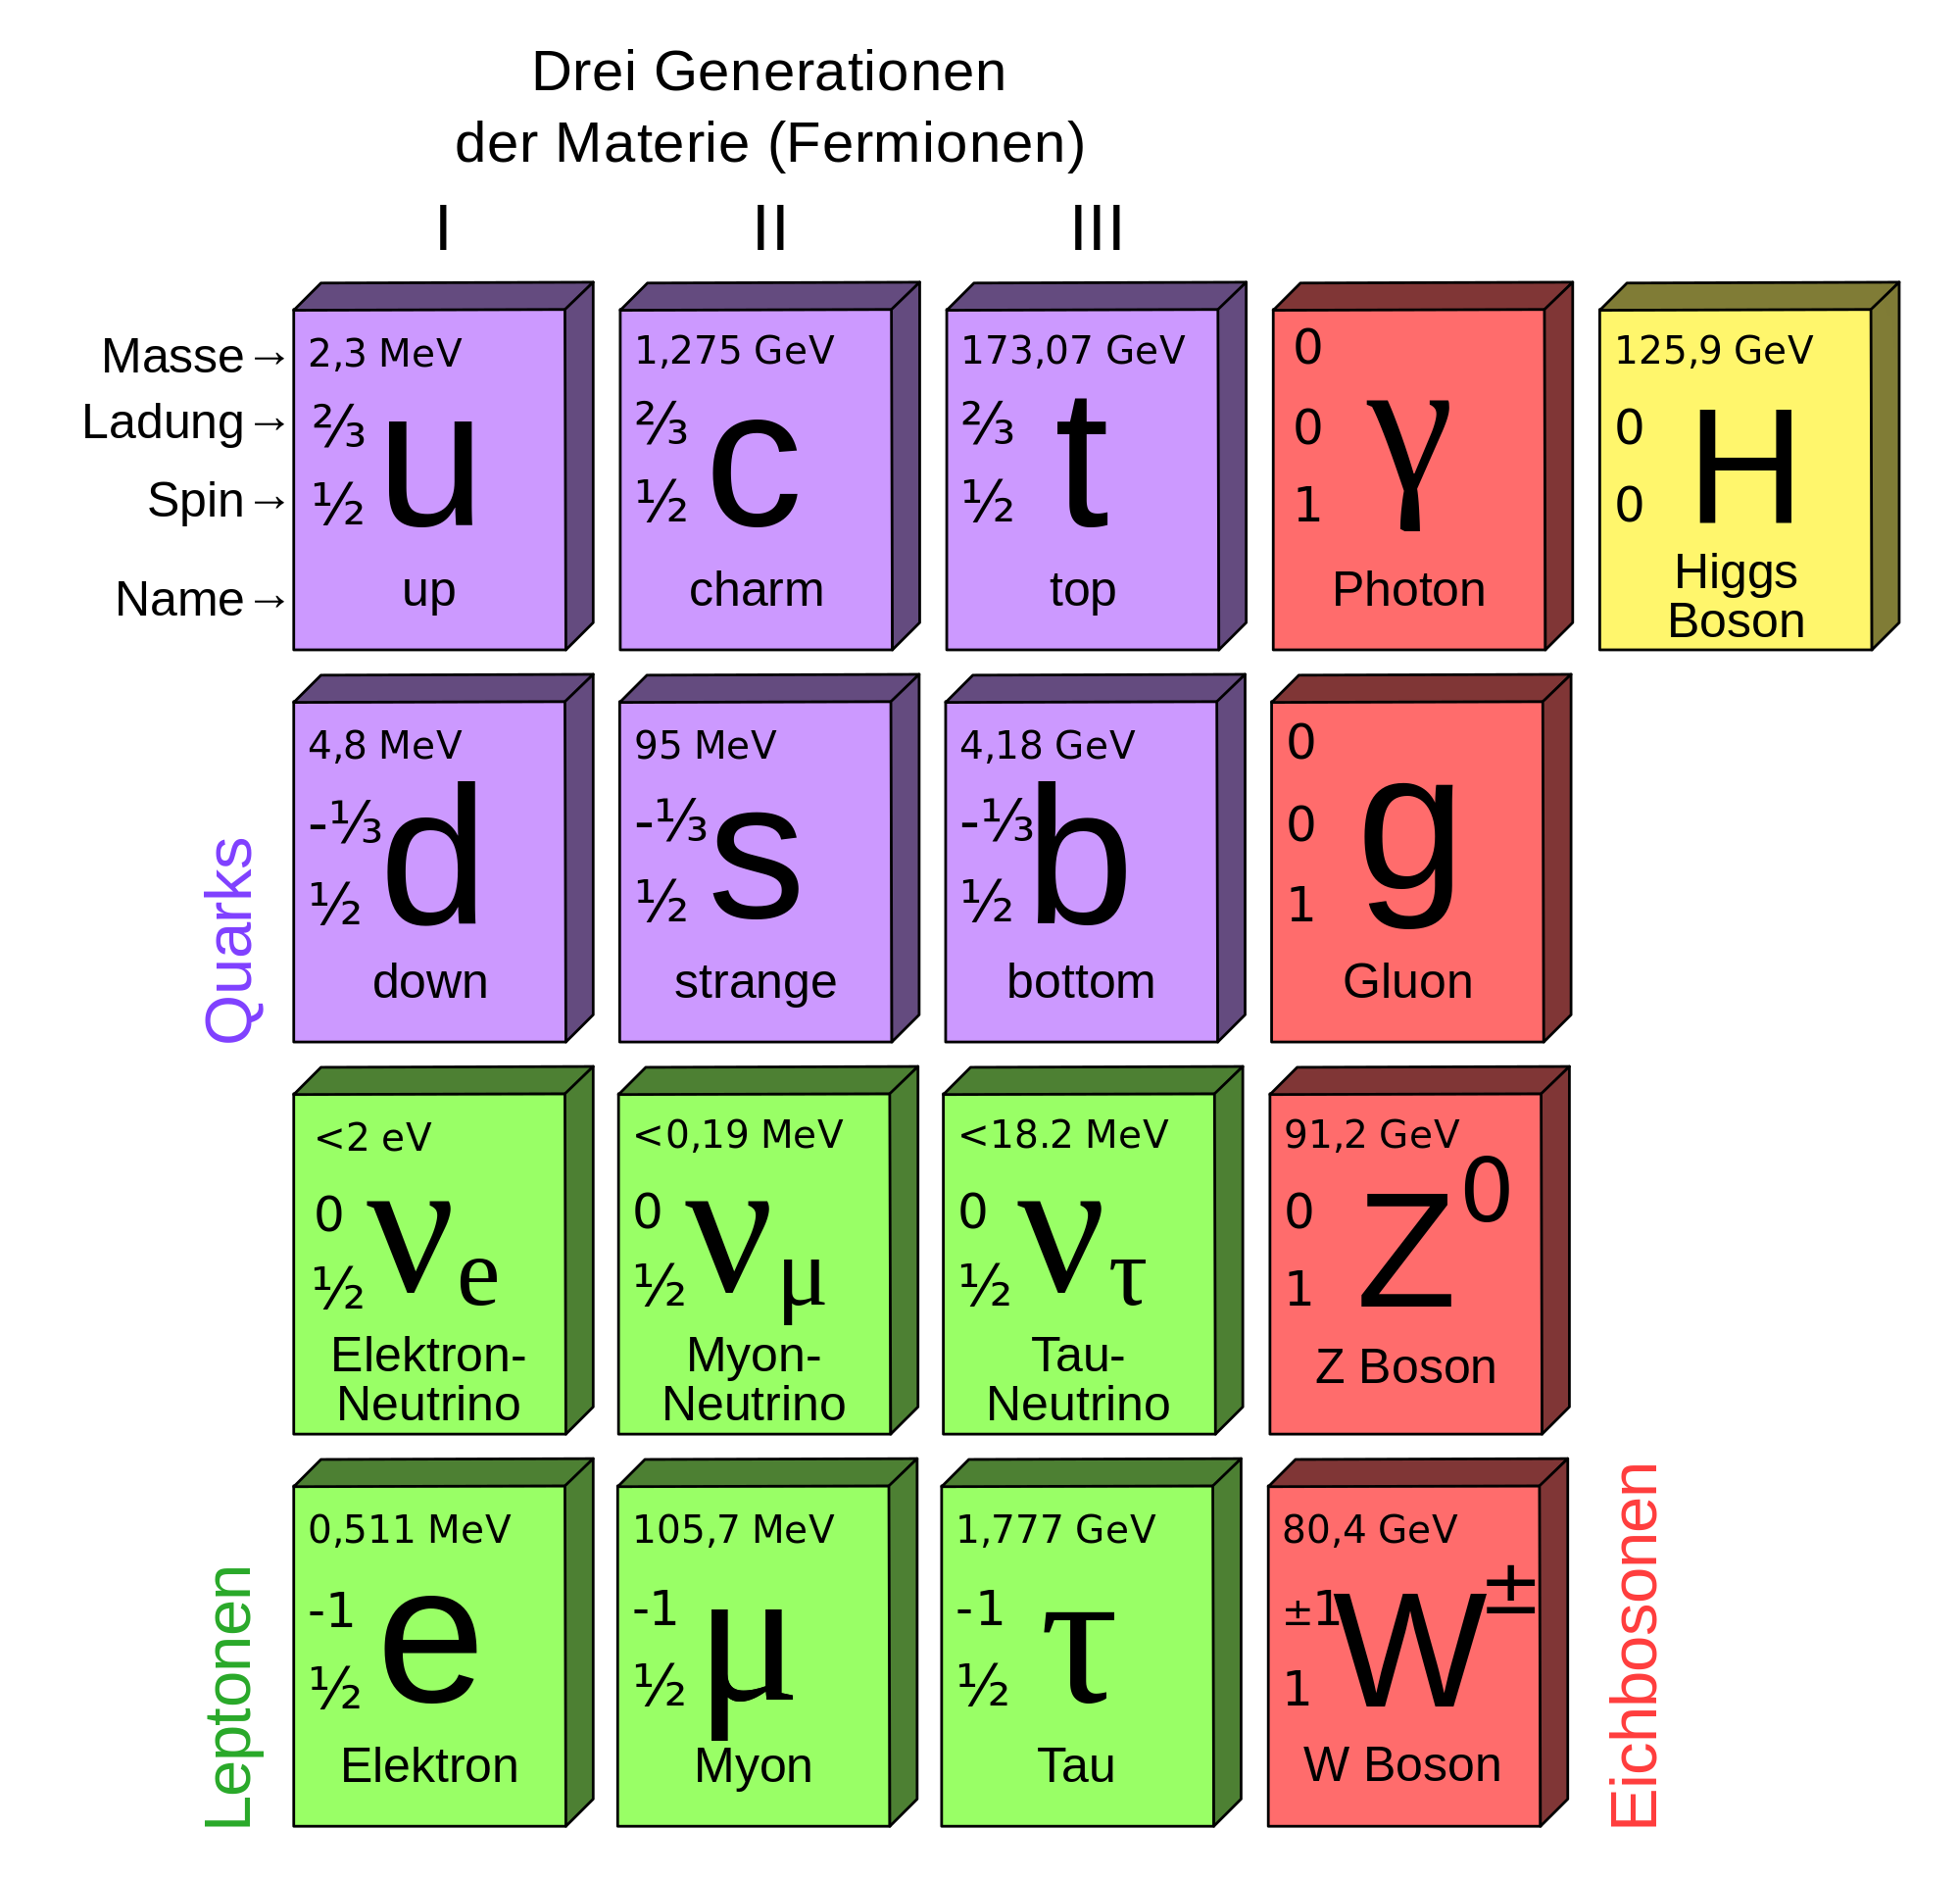
\includegraphics[height=7cm, width=6.7095cm]{Standard_Model_of_Elementary_Particles-de_colorlfull.png}
    \onslide<3>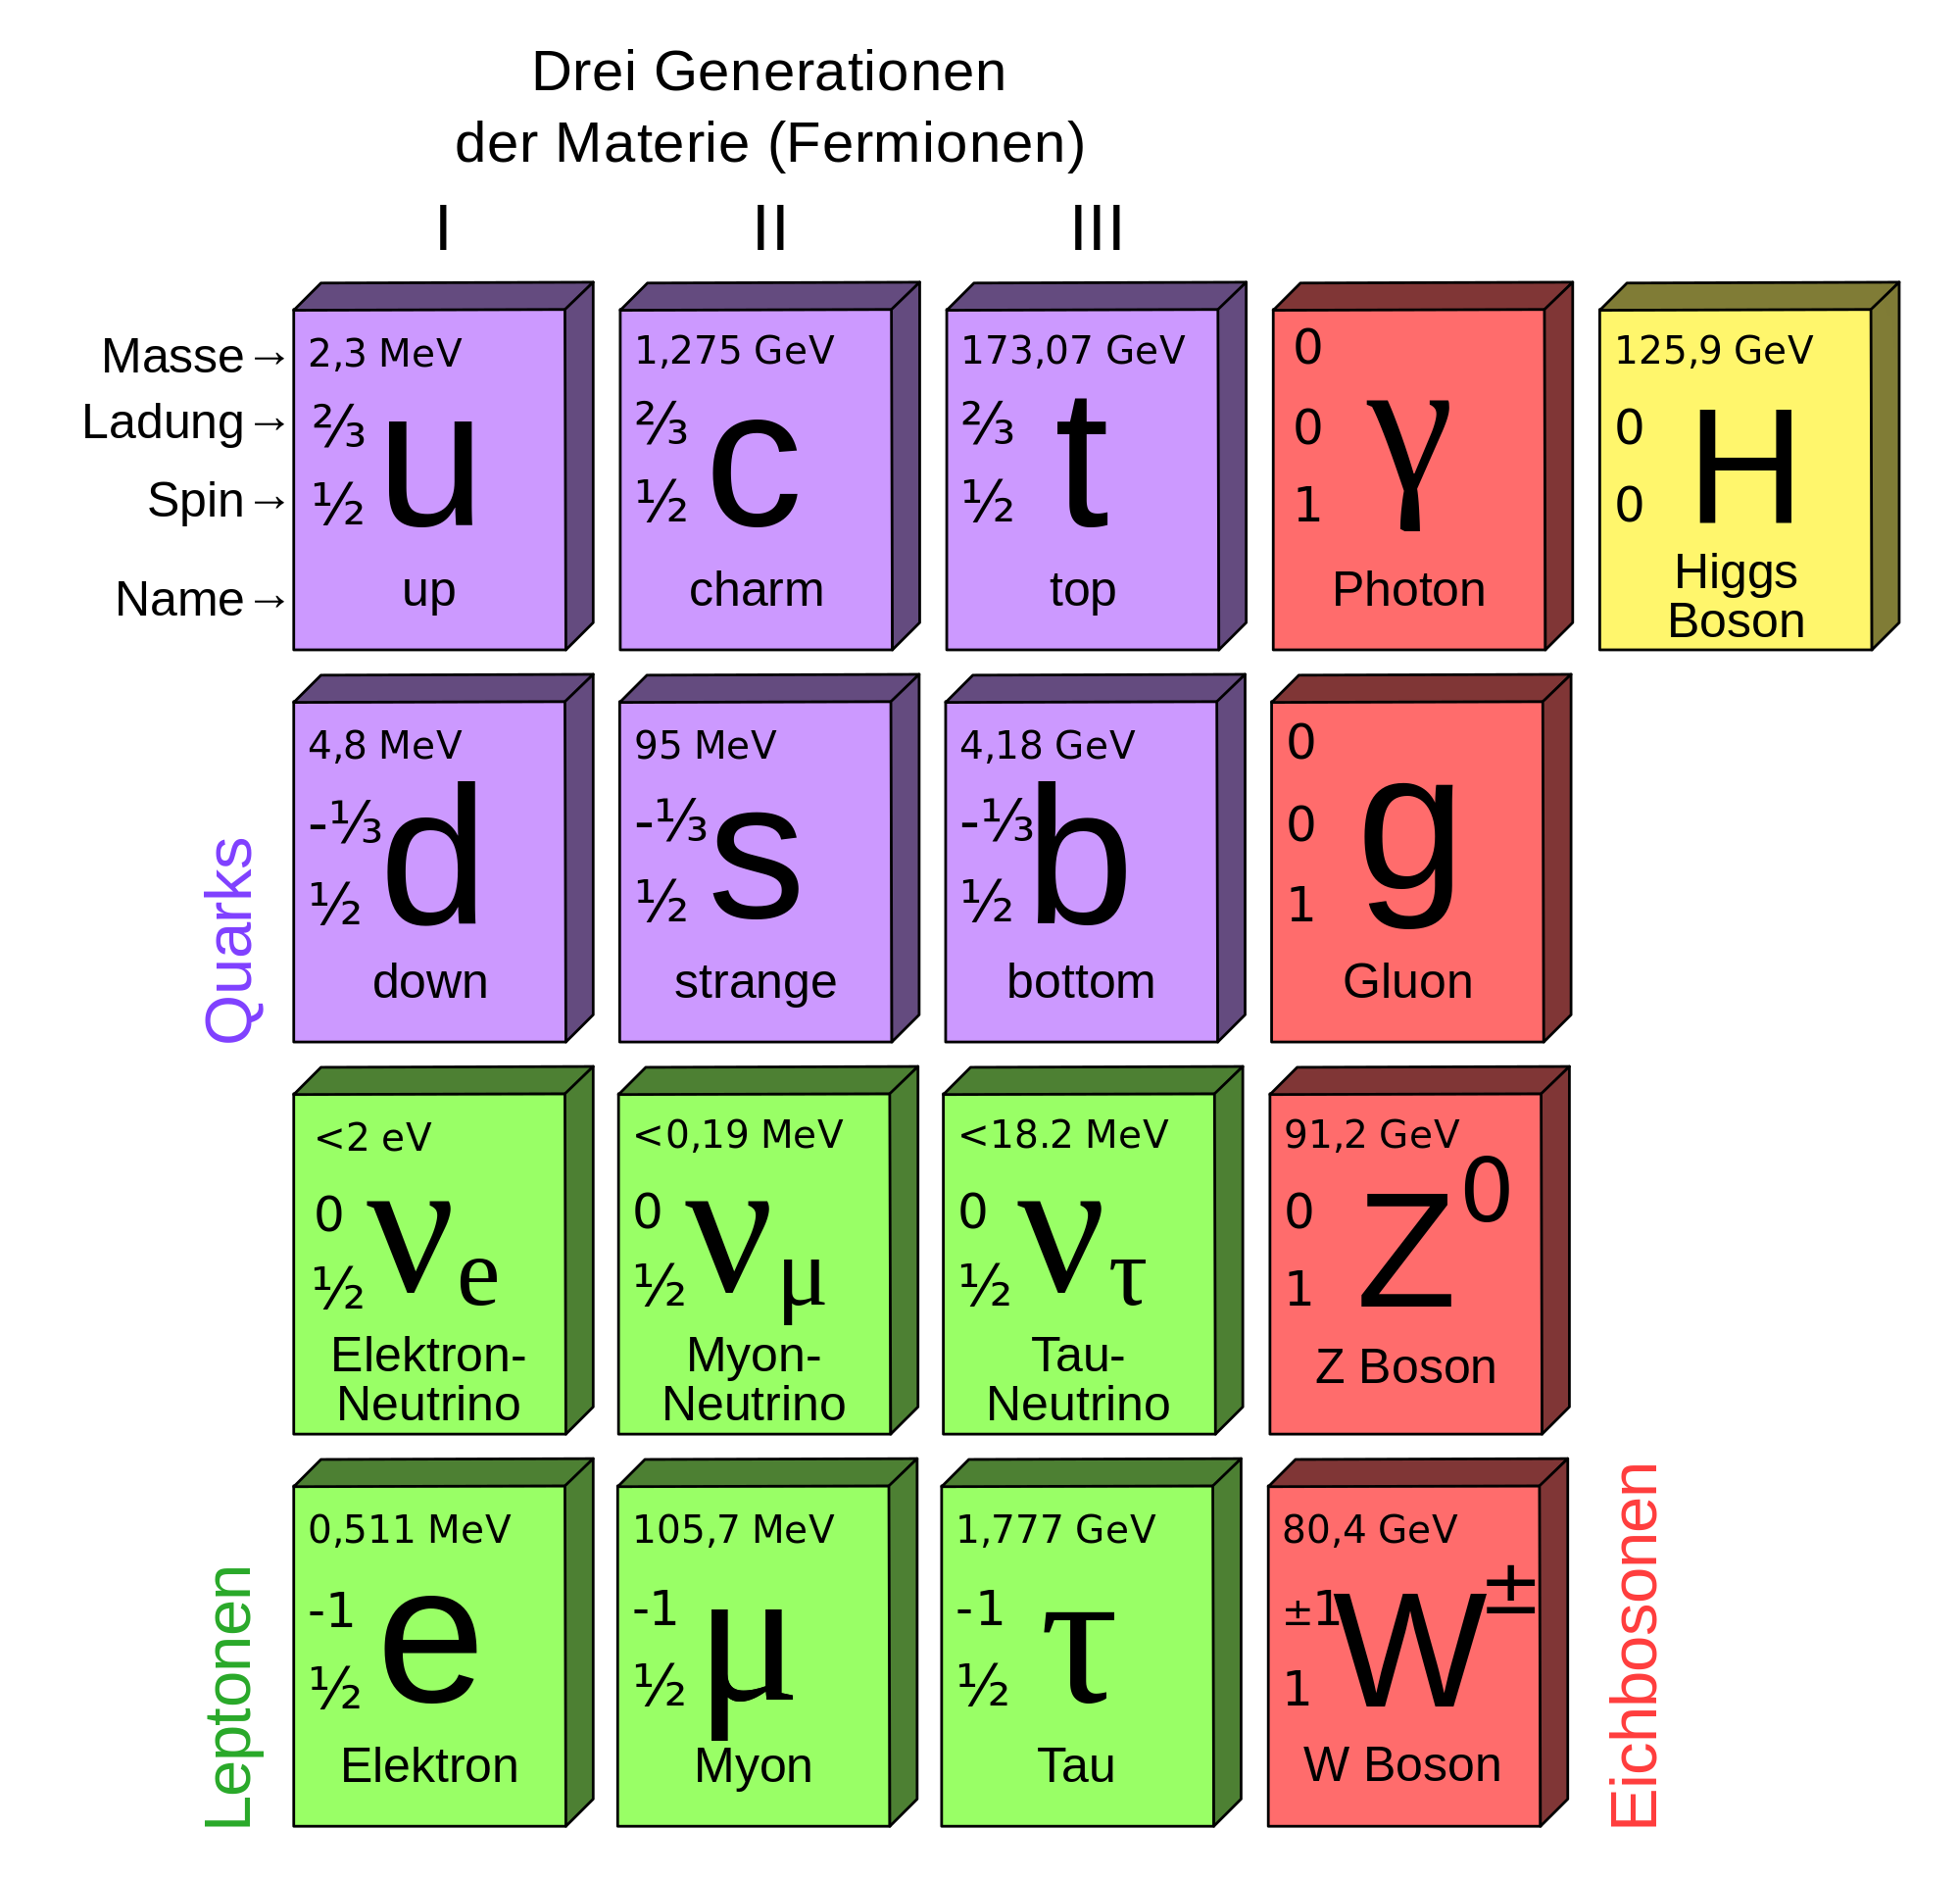
\includegraphics[height=7cm, width=6.7095cm]{Standard_Model_of_Elementary_Particles-de_colorlfull.png}
    \onslide<4->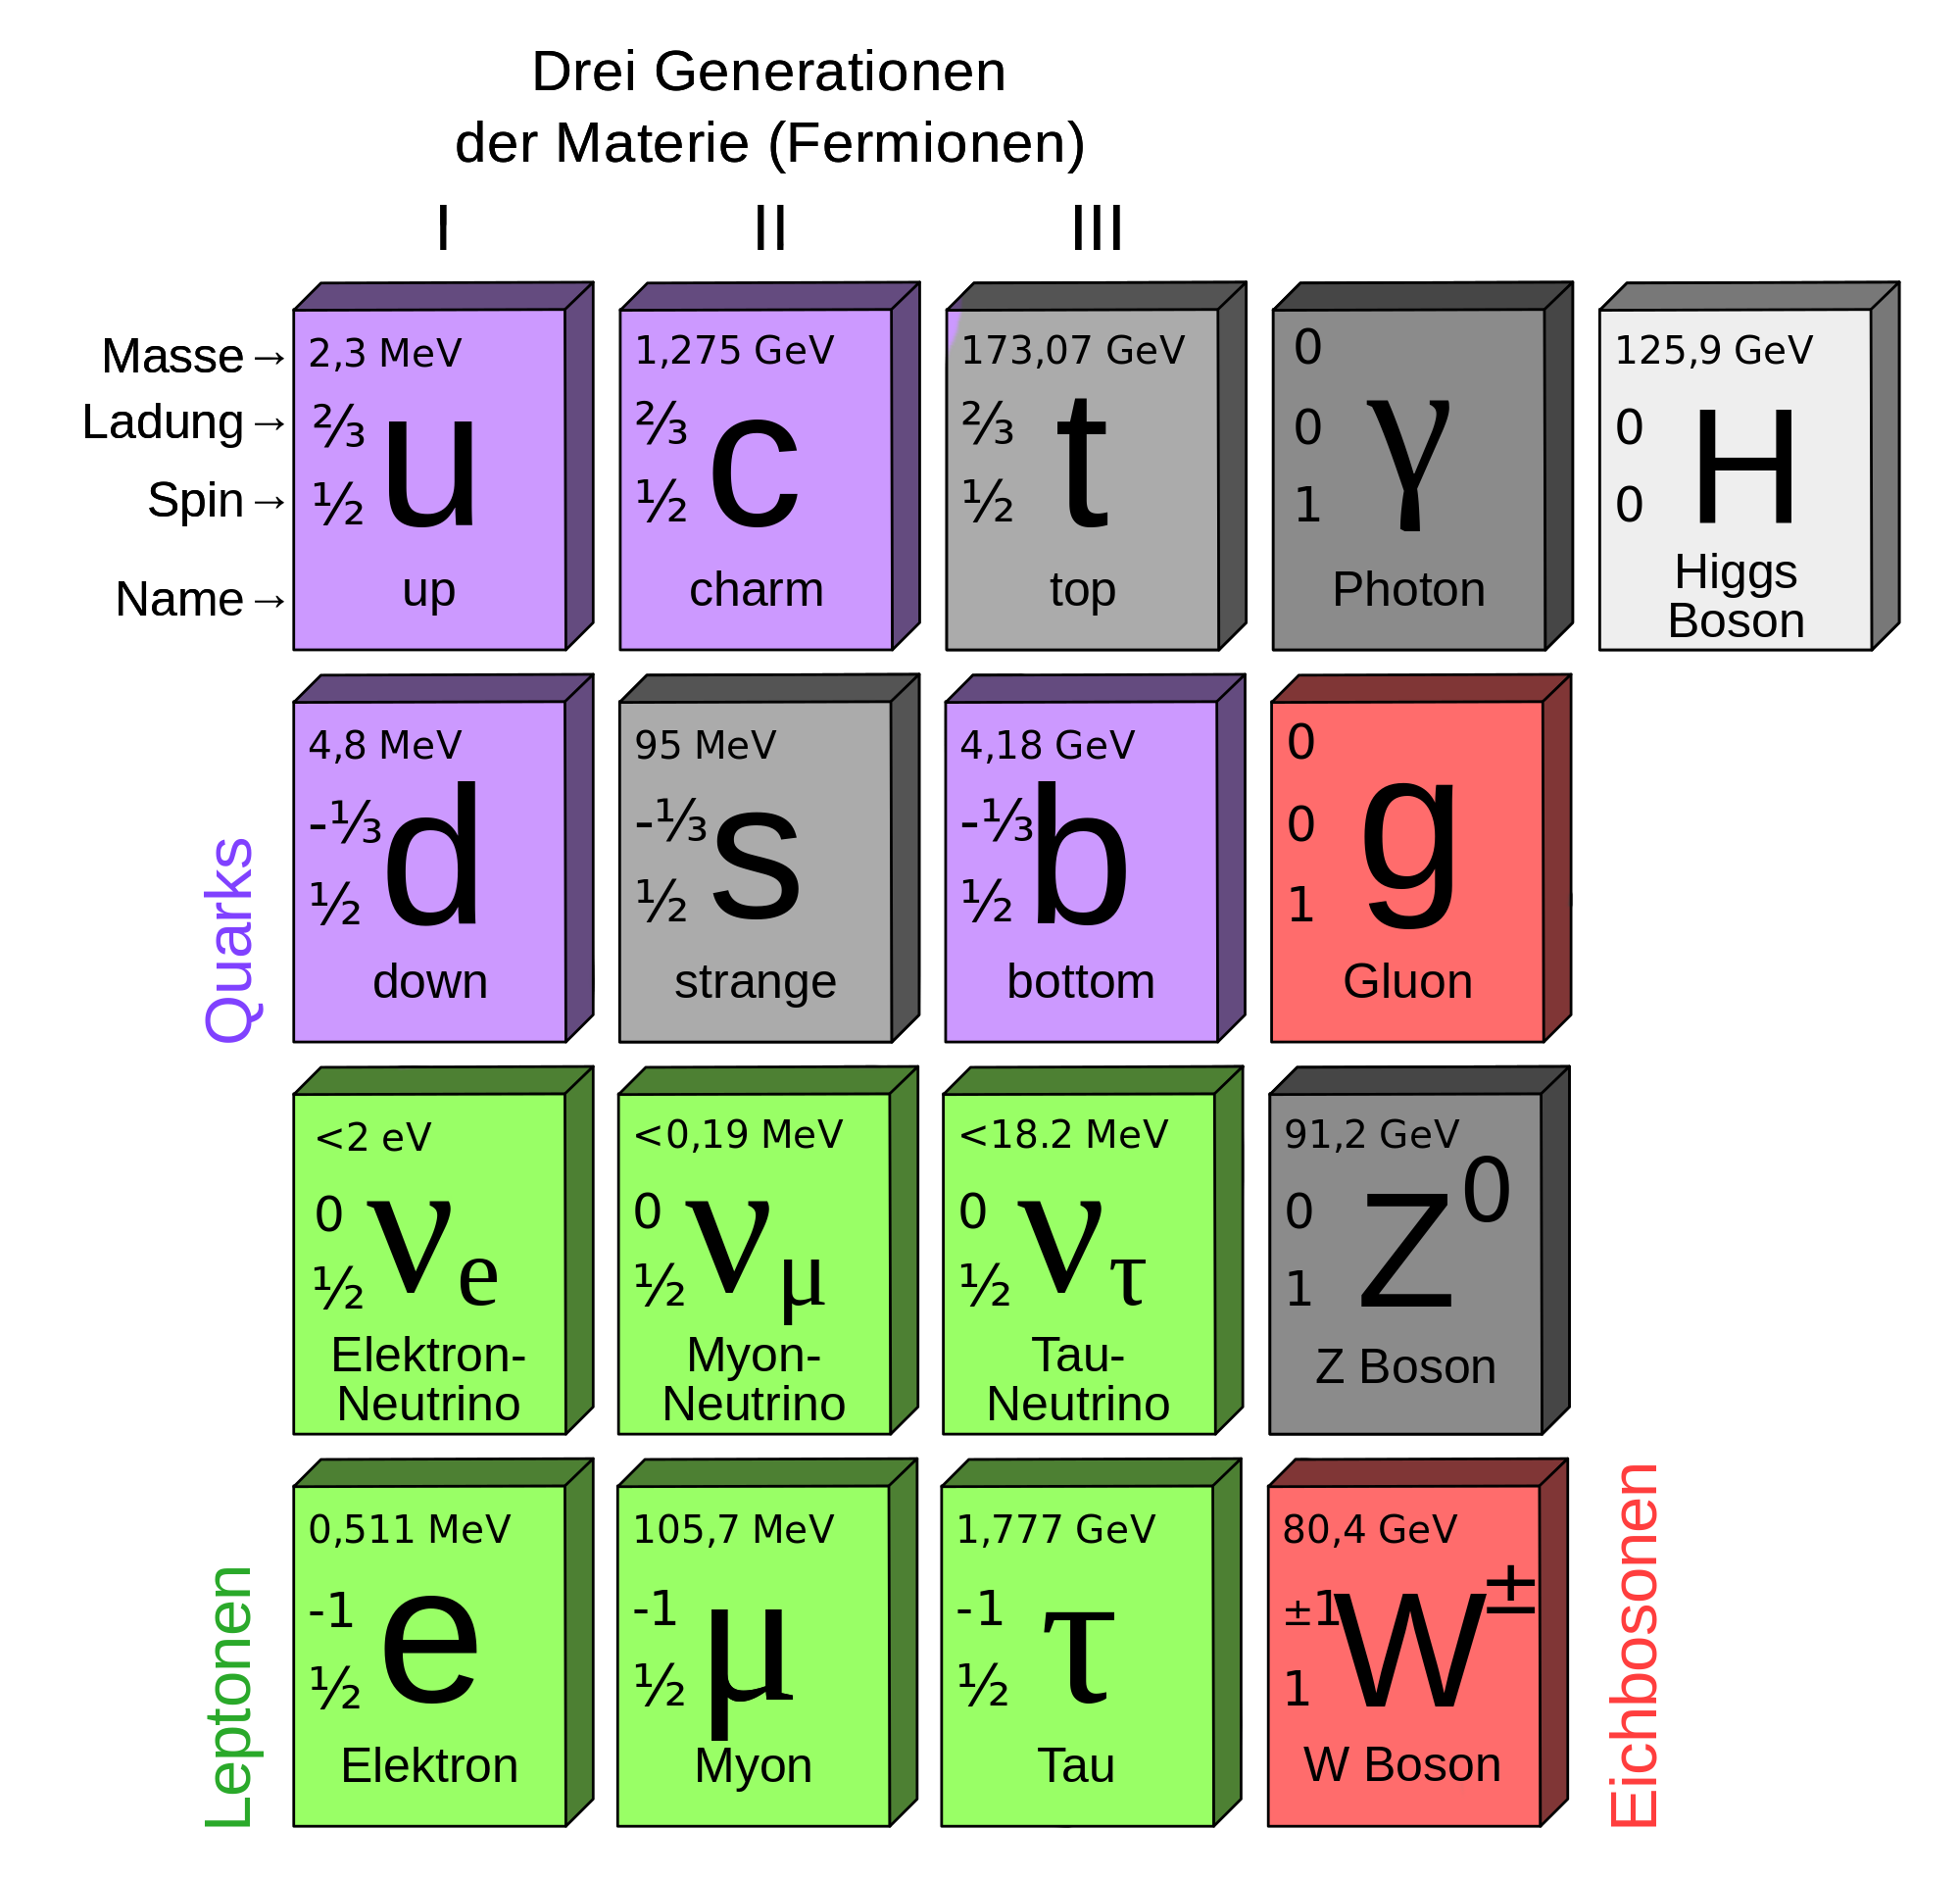
\includegraphics[height=7cm, width=6.7095cm]{Standard_Model_of_Elementary_Particles-de_colorless.png}
  \end{overprint}
    \qquad \onslide<2->\cite{wikipedia}
  \end{minipage}
\end{frame}

\section{Theorie}

\begin{frame}{Inhaltsverzeichnis}
  \tableofcontents[currentsection,currentsubsection,
      hideothersubsections,
      sectionstyle=show/shaded,
  ]\end{frame}

\begin{frame}{Qualitative Beschreibung}
  \frametitle{Qualitative Beschreibung}
  \begin{overprint}
  \onslide<1-2>\begin{figure}
    \centering
    \begin{tikzpicture}
    \begin{feynman}
      \vertex (a1) {\(b\)};
      \vertex[right=1cm of a1] (a2);
      \vertex[right=1cm of a2] (a3);
      %\vertex[right=1cm of a3] (a4) {\(b\)};
      \vertex[right=1cm of a3, label=125:\(V_{cb}\)] (a5);
      \vertex[right=2cm of a5] (a6) {\(c\)};

      \vertex[below=4em of a1] (b1) {\(\overline q\)};
      \vertex[right=1cm of b1] (b2);
      \vertex[right=1cm of b2] (b3);
      \vertex[below=2em of a3] (g1);
      \vertex[left=1.8cm of a6] (g2);
      \vertex[right=1cm of b2] (g5);
      \vertex[left=0.5cm of a6] (g6);
      \vertex[right=1.5cm of g1] (g3);
      \vertex[right=0.8cm of g3] (g4);
      %\vertex[right=1cm of b3] (b4) {\(\overline d\)};
      \vertex[below=4em of a6] (b5) {\(\overline q\)};

      \vertex[above=of a6] (c1) {\(\overline{\nu}_l\)};
      \vertex[above=2em of c1] (c3) {\(l\)};
      \vertex at ($(c1)!0.5!(c3) - (1cm, 0)$) (c2);

      \diagram* {
        {[edges=fermion]
          (b5) -- (b1)
          (a1) -- (a5) -- (a6)
          %(b5) -- (b4) -- (b3) -- (a3) -- (a4) -- (a5) -- (a6),
        },


        (c1) -- [fermion, out=180, in=-45] (c2) -- [fermion, out=45, in=180] (c3),
        (a5) -- [boson, edge label=\(W^{-}\)] (c2),


      };

      \draw [decoration={brace}, decorate] (b1.south west) -- (a1.north west)
            node [pos=0.5, left] {\(\overline B\)};
      %\draw [decoration={brace}, decorate] (c3.north east) -- (c1.south east)
      %      node [pos=0.5, right] {\(\pi^{-}\)};
      \draw [decoration={brace}, decorate] (a6.north east) -- (b5.south east)
            node [pos=0.5, right] {\(D\)};
    \end{feynman}
    \end{tikzpicture}
    \label{fig:feynman2}
  \end{figure}
  \onslide<3->\begin{figure}
    \centering
    \begin{tikzpicture}
    \begin{feynman}
      \vertex (a1) {\(b\)};
      \vertex[right=1cm of a1] (a2);
      \vertex[right=1cm of a2] (a3);
      %\vertex[right=1cm of a3] (a4) {\(b\)};
      \vertex[right=1cm of a3, label=125:\(V_{cb}\)] (a5);
      \vertex[right=2cm of a5] (a6) {\(c\)};

      \vertex[below=4em of a1] (b1) {\(\overline q\)};
      \vertex[right=1cm of b1] (b2);
      \vertex[right=1cm of b2] (b3);
      \vertex[below=2em of a3] (g1);
      \vertex[left=1.8cm of a6] (g2);
      \vertex[right=1cm of b2] (g5);
      \vertex[left=0.5cm of a6] (g6);
      \vertex[right=1.5cm of g1] (g3);
      \vertex[right=0.8cm of g3] (g4);
      %\vertex[right=1cm of b3] (b4) {\(\overline d\)};
      \vertex[below=4em of a6] (b5) {\(\overline q\)};

      \vertex[above=of a6] (c1) {\(\overline{\nu}_l\)};
      \vertex[above=2em of c1] (c3) {\(l\)};
      \vertex at ($(c1)!0.5!(c3) - (1cm, 0)$) (c2);

      \diagram* {
        {[edges=fermion]
          (b5) -- (b1)
          (a1) -- (a5) -- (a6)
          %(b5) -- (b4) -- (b3) -- (a3) -- (a4) -- (a5) -- (a6),
        },


        (c1) -- [fermion, out=180, in=-45] (c2) -- [fermion, out=45, in=180] (c3),
        (a5) -- [boson, edge label=\(W^{-}\)] (c2),

        (a2) -- [gluon] (g1)
        (b2) -- [gluon] (g1)
        (g1) -- [gluon] (g2)
        (g5) -- [gluon] (g3)
        (g3) -- [fermion, half left] (g4)
        (g4) -- [fermion, half left] (g3)
        (g4) -- [gluon] (g6)

      };

      \draw [decoration={brace}, decorate] (b1.south west) -- (a1.north west)
            node [pos=0.5, left] {\(\overline B\)};
      %\draw [decoration={brace}, decorate] (c3.north east) -- (c1.south east)
      %      node [pos=0.5, right] {\(\pi^{-}\)};
      \draw [decoration={brace}, decorate] (a6.north east) -- (b5.south east)
            node [pos=0.5, right] {\(D\)};
    \end{feynman}
    \end{tikzpicture}
    \label{fig:feynman2}
  \end{figure}
  \end{overprint}


  \begin{itemize}
    \item<2-> Schwache Wechselwirkung: $b \to c$ mit $ \lvert V_{cb} \rvert = \SI{40.49+-0.97e-3}{}$ \cite{Bigi2017441}
    \item<3-> Starke Wechselwirkung: Zunahme der starken Kopplungskonstante $\alpha_\text{s}$ bei geringer werdenden Impulsüberträgen
    \item[→]<4-> Keine Entwicklung in $\alpha_\text{s}$ als Störungstheorie mehr möglich.
    \item[→]<5-> Quantitative Aussagen weiterhin möglich durch Formfaktoren
  \end{itemize}

\end{frame}

\begin{frame}{Parametrisierung des Matrixelementes}
  \begin{itemize}
    \setlength\itemsep{1em}
    \item<2-> Matrixelement: $M = \bra{D \, l \, \overline{\nu}_l} \, H \, \ket{ \overline{B} } = \bra{ l \, \overline{\nu_l}} \, H_\text{lep} \, \ket{0}  \bra{D} \, H_\text{had} \, \ket{ \overline{B} } $
    \item<3-> Beschreibung des hadronischen Matrixelementes durch V-A-Strom: \\ $\bra{D} \, H_\text{had} \, \ket{ \overline{B} } = \bra{D} \, \overline{c} \gamma_\mu (1 - \gamma_5) b \, \ket{ \overline{B} } = \bra{D} \underbrace{\overline{c} \gamma_\mu b \, }_{= V_\mu} \ket{\overline{B} } - \bra{D} \, \underbrace{ \overline{c} \gamma_\mu \gamma_5 b}_{= A_\mu}\, \ket{ \overline{B} }$
    \item<3-> Parametrisierung des Matrixelementes durch $p^B$, $p^D$, $q^2 = (p^B - p^D)^2$
    \item<4-> Erhaltung der Parität in QCD: $\bra{D} A_\mu \ket{\overline{B}} = 0$
    \item<5-> Formfaktoren: $\bra{D} \, V_\mu \, \ket{\overline{B}} = f_+(q^2)(p^B + p^D)_\mu + f_{-}(q^2)(p^B - p^D)_\mu$
  \end{itemize}
\end{frame}


\begin{frame}{Parametrisierung des Matrixelementes}
  \begin{equation}
    \frac{\mathrm{d} \Gamma}{\mathrm{d} q^2} \left(\overline{B} \to D l \overline{\nu}_l \right) = \frac{\eta_\text{EW}^2 G_\text{F}^2 \lvert V_{cb} \rvert^2 m_B \sqrt{\lambda} }{192 \pi^3} \left( 1 - \frac{m_l^2}{q^2} \right)^2 \left( c_+^l f_+(q^2)^2 + c_0^l f_0(q^2)^2 \right)
  \end{equation}
  mit den Abkürzungen
  \begin{align*}
    c_+^l &= \frac{\lambda}{m_B^4} \left( 1 + \frac{m_l^2}{2 q^2} \right) \\
    c_0^l &= \left(1 - \frac{m_D^2}{m_B^2} \right)^2 \frac{3 m_l^2}{2 q^2} \\
    \lambda &= (q^2 - m_B^2 - m_D^2)^2 - 4 m_B^2 m_D^2 \\
    f_0(q^2) &= f_+(q^2) + f_{-}(q^2) \frac{q^2}{m_B^2 - m_D^2}.
  \end{align*}
  \cite{PhysRevD.94.094008}
\end{frame}

\begin{frame}{Kinematische Größen}
  \begin{itemize}
    %\setlength\itemsep{1em}
    \item<2-> Impulsübertrag: $m_l^2 \leq q^2 \leq (m_B - m_D)^2$
    \item<3-> Alternative Parametrisierungen:
  \end{itemize}
  \begin{align*}
    \onslide<4->{w(q^2) &= \frac{m_B^2 + m_D^2 - q^2}{2 m_B m_D}\\[10pt]}
    \onslide<5->{z(q^2) &= \frac{\sqrt{w+1}-\sqrt{2}}{\sqrt{w+1}+\sqrt{2}}}
  \end{align*}
\end{frame}


\begin{frame}{Kinematische Größen - z-Parametrisierung}
  \begin{minipage}{5cm}
    \begin{align*}
      z(q^2) &= \frac{\sqrt{w+1}-\sqrt{2}}{\sqrt{w+1}+\sqrt{2}}
    \end{align*}
  \end{minipage}%
  \begin{minipage}{10cm}
    \begin{figure}
      \centering
      \includegraphics[width=\textwidth]{plot_z_2.pdf}
    \end{figure}
  \end{minipage}
\end{frame}

\section{Fit}

\begin{frame}{Inhaltsverzeichnis}
  \tableofcontents[currentsection,currentsubsection,
      hideothersubsections,
      sectionstyle=show/shaded,
  ]\end{frame}

\begin{frame}
    Hier fitte ich.
\end{frame}

\begin{frame}
    Weitere Fits.
\end{frame}

\section{Zusammenfassung}

\begin{frame}{Inhaltsverzeichnis}
  \tableofcontents[currentsection,currentsubsection,
      hideothersubsections,
      sectionstyle=show/shaded,
  ]\end{frame}

\begin{frame}
    Hier fasse ich zusammen.
\end{frame}

\section{Quellen}

\begin{frame}{Quellen}
  \tableofcontents[currentsection,currentsubsection,
      hideothersubsections,
      sectionstyle=show/shaded,
  ]\end{frame}

\begin{frame}
    \printbibliography
\end{frame}

\section{Diskussion}

\begin{frame}{Inhaltsverzeichnis}
  \tableofcontents[currentsection,currentsubsection,
      hideothersubsections,
      sectionstyle=show/shaded,
  ]\end{frame}

\end{document}
